\documentclass[11pt, norsk]{article}
%\usepackage[latin1]{inputenc}
\usepackage[T1]{fontenc}
\usepackage[utf8]{inputenc}
\usepackage[norsk]{babel}   % S P R A A K
% \usepackage{graphicx}    % postscript graphics
\usepackage{amssymb, amsmath, amsthm, amssymb} % symboler, osv
\usepackage{mathrsfs}
\usepackage{url}
\usepackage{thmtools}
\usepackage{enumerate}  % lister $  
\usepackage{float}
\usepackage{tikz}
\usepackage{tikz-cd}
\usetikzlibrary{calc}
%\usepackage{tikz-3dplot}
\usepackage{subcaption}
\usepackage[all]{xy}   % for comm.diagram
\usepackage{wrapfig} % for float right
\usepackage{hyperref}
\usepackage{mystyle} % stilfilen      

%\usepackage[a5paper,margin=0.5in]{geometry}


\begin{document}
\title{Notater}
\author{Fredrik Meyer}
\maketitle 

\subsection{Tautologisk linjebunt på $\PP^n$}

Vi kan definere en tautologisk linjebunt på $\PP^n$. Dette er en bunt hvis fiber over et punkt $p$ er linjen i $\Aa^{n+1}$ utspent av (de homogene koordinatene til) $p$. La $q \in \langle p \rangle$ bety at $q$ er med i spennet av $p$. Da er
$$
\mathscr T := \{ (q,p) \in \Aa^{n+1} \times \PP^n \mid q \in \langle p \rangle \}.
$$
Ved å regne overgangsfunksjoner kan en se at $\mathscr T \simeq \OO_{\PP^n}(-1)$.

Det finnes også andre måter å se dette på, eksempelvis slik Mike Eastwood forklarte det på siste forelesning, men det har jeg glemt av nå (!!). 

\subsection{Embedding Grassmannian}

Grassmannian har en tautologisk 
Da vil $\wedge^k \mathscr E$ være en linjebunt på Grassmannian, og seksjonene vil være utspent av alle minorene. Så dette er linjebunten Plücker-embeddingen svarer til.

\subsection{Topologien til SR-skjemaer}

La $X=\PP(\Delta)$ være et Stanley-Reisner-skjema. La $f=(f_0,\ldots,f_n)$ være $f$-vektoren, det vil si, antall $f_i$ er antall $i$-dimensjonale fasetter i $\Delta$. Da er $h^i(\PP_\C(\Delta),\C)=f_i$ om $i$ er jevn, og $0$ ellers. Dette er fordi $X$ har strukturen til et CW-kompleks med bare celler i jevne grader.

\subsection{Kotangentkohomologi på en oppblåsning}

La $\pi:\widetilde X \to X$ være oppblåsningen av en glatt flate $X$ i et punkt $P$. La $E \simeq \PP^1$ være den eksepsjonelle divisoren. Vi ønsker å beregne kohomologien $H^i(\Omega_{\widetilde X/k}^1)$ gitt kjennskap til kohomologien til $X$.

Et standard teorem sier at vi har en eksakt sekvens
$$
\pi^\ast \Omega^1_{X/k} \to \Omega^1_{\widetilde X/k} \to \Omega^1_{\widetilde X/X} \to 0.
$$

Påstanden er at denne er venstre-eksakt også. Siden $\widetilde X \bs E \simeq X \bs P$ er den første pilen en isomorfi utenfor $E$ (og dermed er høyre-leddet også null). Om vi er på $Q \in E$, har vi at $\mathscr G = {\pi^\ast \Omega_{X/k}^1}$ er null langs $E$, siden stilken $\mathscr G_Q=\Omega_{f(x)/k}^1$, og kotangentknippet over et punkt er null.

Legg også merke til at $\Omega^1_{\widetilde X/X}=i_\ast \OO_{\PP^1}(-2)$ siden $E \simeq \PP^1$ og knippet er null utenfor $E$ (her er $i:\PP^1 \to \widetilde X$ inklusjonen). Dermed har vi sekvensen
$$
0 \to \pi^\ast \Omega^1_{X/k} \to \Omega^1_{\widetilde X/k} \to i_\ast \mathscr O_{\PP^1} (-2) \to 0.
$$

Vi har også at $H^i(\pi^\ast \Omega^1_{X/k})= H^i(\Omega_{X/k}^1)$ (se beviset for Zariskis hoved-teorem i Hartshorne).

Dermed har vi at $H^0(\Omega_{\widetilde X/k}^1) = H^0(\Omega_{X/k}^1)$. For å regne ut de andre kohomologigruppene trenger vi mer presis informasjon om $X$. Så anta $X= \PP^2$. Da følger det fra Euler-sekvensen at $H^i(\Omega_{X/k}^1)$ er null for $i=0,2$ og $1$ for $i=1$. Dermed følger det at $H^i(\Omega_{\widetilde X/k}^1)$ er null for $i=0,2$ og $2$ for $i=1$.

Så å blåse opp i et punkt øker $H^1$ med én.

\subsection{Dobbel overdekning av $\PP^2$ ramifisert i gitt kurve}

Gitt et homogent polynom $f(x,y,z)$ i $H^0(\PP^2,\OO_{\PP^2}(2n))$, konstruerer vi en flate som er en dobbel overdekning av $\PP^2$, ramifisert i kurven definert ved dette polynomet.

Den naive løsningen funker, men virker upraktisk å jobbe med. Betrakt nullpunktsmengden $X$ til $f-u^2$ i $\PP(1,1,1,n)$. Dette er en veldefinert varietet, siden polynomet er homogent i denne graderingen.  Vi har en avbildning $\pi:X \to \PP^2$ gitt ved $(x:y:z:u) \mapsto (x:y:z)$. Dette er i utgangspunktet kun en rasjonal avbildning, men formen på ligningen viser at avbildningen er veldefinert: for anta at vi blir sendt til ``punktet'' $(0:0:0)$. Da er $x=y=z=0$, som tvinger $u=0$. Men dette er absurd, så avbildningen må være en morfi.

Anta at $P \not \in V(f) \in \PP^2$. Da er $f(P) \neq 0$. Dermed får vi at fiberen $\pi^{-1}(P)$ består av to forskjellige punkter. Om $f(P)=0$, får vi kun ett punkt i fiberen.

Det eneste singulære punktet i $\PP(1,1,1,3)$ er $(0:0:0:1)$, og dette punktet ligger ikke på $X$. Det følger at $X$ er glatt. Faktisk er $\PP(1,1,1,3)$ isomorf med den projective kjeglen over $\nu_3(\PP^2)$ (den tredje Veronese-embeddingen av $\PP^2$).

Legg merke til at avbildnigen $\pi:X \to \PP^2$ er en affin avbildning (i betydningen at $\pi^{-1}(U_i)$ er affin for $i=0,1,2$). Dette impliserer (oppgave III.8.2 i Hartshorne) at $H^i(X,\OO_X) = H^i(\PP^2,\pi_\ast \OO_X)$ for $i \geq 0$. Derfor ønsker vi å regne ut $\pi_\ast \OO_X$.

Vi har at den homogene koordinatringen til $X$ er gitt ved $S = k[x,y,z,u]/(f-u^2)$, med gradene $(1,1,1,3)$. La $T=k[x,y,z]$ være den homogene koordinatringen til $\PP^2$. Da har vi at
$$
S = T \oplus u T (-3)
$$
som en gradert $T$-modul. 

(dette burde implisere at $\pi_\ast \OO_X = \OO_{\PP^2} \oplus \OO_{\PP^2}(-3)$.)

\subsection{Utregninger på $D_4$-singulariteten}

Vi skal blåse opp singulariteten $\{ x^2+y^3+z^3=0 \} \subseteq \Aa^3$.  Oppblåsningen ligger i $\Aa^3_{xyz} \times \PP^2_{abc}$, og har ligninger
$$
x^2+y^3+z^3=0, ay=bx, az=cx, bz=cy,
$$
hvor $a,b,c$ er homogene koordinater på $\PP^2$. Vi har tre kart å betrakte, og disse er gitt ved å sette $a=1,b=1,c=1$.

Setter vi $a=1$, kan vi eliminere $y$ og $z$, og vi ender opp med ligningen
$$
\{x^2+b^3x^3+c^3x^3=0\} \subseteq \Aa^1_x \times \Aa^2_{bc}.
$$

Denne splitter som $\{x^2 =0\} \cup \{ 1+x(b^3+c^3) = 0\}$. En rask utregning viser at flaten er glatt, og ikke snitter den eksepsjonelle i dette kartet.

Nå setter vi $b=1$, og vi kan eliminere $x$ og $z$. Vi ender opp med ligningen $y^2(a^2+y+c^3y)=0$. Den propre transformen er en singular flate med tre dobbeltpunkter når $a=y=0$ og $c^3=-1$. Dette kan ses ved å gjøre et variabelskifte: vi setter $c'=c+1$, og finner at ligningen nå tar formen
$$
a^2+yc(c^2-3c+3)=0.
$$
Den siste faktoren er en enhet i $k[[a,y,c]]$, så denne kan ses bort fra i kompletteringen. Dette er ligningen til et rasjonalt dobbeltpunkt, og vi vet at én oppblåsning til holder for å løse opp dette.

I kartet $c=1$, får vi samme resultat, bare med andre koordinater.

$$
\xymatrix{
	\widetilde X \ar[r] \ar[d]^\sigma & \Aa^3 \times \PP^2 \ar[dl]^{\pi_1} \\
	X
}
$$

Dermed ser vi at oppblåsningen har tre singulariteter i koordinatene $(0,0,0) \times (0:1:\zeta^i)$, hvor $\zeta^3=-1$ og $i=0,1,2$. Nok en oppblåsning i hver av disse tre singularitetene glatter flaten. De eksepsjonelle krysser på denne måten:

\begin{center}
\begin{tikzpicture}
\draw (0,0) -- (4,0);
\draw (1,-1) -- (1,1);
\draw (2,-1) -- (2,1);
\draw (3,-1) -- (3,1);
\end{tikzpicture}
\end{center}

Den horisontale linjen er den eksepsjonelle fra den første oppblåsningen. De tre andre linjene kommer fra oppblåsningen av dobbeltpunktene. De kan ikke snitte hverandre siden de blir sendt til forskjellige punkter i nedblåsningen.

Lager vi dualgrafen til snittgrafen over, får vi dette bildet (dualgrafen er gitt ved at hjørnene svarer til eksepsjonelle divisorer og kantene svarer til snitt):

\begin{center}
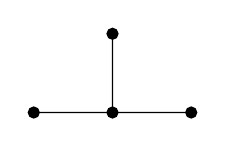
\begin{tikzpicture}
\filldraw
(0,0) circle (2pt)
(-1,0) circle (2pt) 
(1,0) circle (2pt)
(0,1) circle (2pt)
(0,0) -- (0,1)
(0,0) -- (-1,0)
(0,0) -- (1,0);
\end{tikzpicture}
\end{center}

Dette er Dynkin-diagrammet $D_4$. 

Vi kan gjøre mer. Alle du Val-singularitetene er rasjonale dobbeltpunkter, så det burde være mulig å finne en parametrisering av $D_4$, det vil si en rasjonal avbildning $\Aa^2 \rmap X$. En måte å gjøre dette på, er å projisere fra $X$ til planet $z=-1$ gjennom det singulære punktet $(0,0,0)$. Dette gir en rasjonal avbildning, siden linjen mellom $(0,0,0)$ og punktet $x \in X$ treffer det singulære punktet dobbelt, og $x$ én gang.

Eksplisitt får vi avbildningen gitt ved
$$
\Aa^2 \ni (a,b) \mapsto \left( \frac{a^3}{1-b^3}, \frac{a^2b}{1-b^3}, \frac{-a^2}{1-b^3}\right) \in X.
$$

Dette er en birasjonal avbildning. Vi ser at hele $b$-aksen avbildes på origo, men for linjene $\{b^3=1\}$ er ikke avbildnigen definert.

Q: Er det sant at det ikke finnes noen birasjonal surjektiv morfi $\Aa^2 \to X$? 

\subsection{Bruke Hurwitz og overdekninger}

Her er et eksempel på bruk av Hurwitz' formel for å regne ut genusen til en kurve. La $X$ være kurven i $\PP^1 \times \PP^1$ gitt ved $(x_0^2+x_1^2)(y_0^2+y_1^2)=x_0x_1y_0y_1$. Betrakt (restriksjonen av) projeksjonen ned på $\PP^1$. Dette gir en surjektiv avbildning $X \to \PP^1$ av grad $2$. Dermed sier Hurwitz at $2g-2=2(0-2)+\deg R$, hvor $R$ er ramifikasjonsdivisoren. Dette er en divisor på $X$ som består av punktene hvor avbildningen ikke er $2:1$. 

Man kan regne ut graden til denne på følgende vis: vi regner lokalt ved å sette $x_0=y_0=1$. Størrelsen på fiberen er gitt ved å løse en andregradsligning i $y_1$, og da er diskriminantlokuset gitt ved diskriminanten til denne ligningen, som er av grad $4$. Dermed får vi at $2g-2=-4+4$, så $g=1$.

Et annet eksempel på bruk av overdekninger er følgende: se på $\PP^3 \times \PP^1$. la $X$ være en generisk medlem i $|\OO_{\PP^3 \times \PP^1}(-2,d)|$, og igjen betrakt projeksjonen ned på $\PP^3$. Dette er en $2:1$-avbildning igjen, og ved essensielt samme formel har vi nå at $\deg K_X = 2 \deg  K_{\PP^3} + d$, hvor $d$ igjen blir graden til ramifikasjonsdivisoren. Med andre ord, ønsker vi at $X$ skal bli Calabi-Yau, må vi velge $d=8$. Dette svarer da til en velkjent Calabi-Yau: en dobbel overdekning av $\PP^3$ ramifisert i en oktikk.

\end{document}